% Options for packages loaded elsewhere
\PassOptionsToPackage{unicode}{hyperref}
\PassOptionsToPackage{hyphens}{url}
\PassOptionsToPackage{dvipsnames,svgnames,x11names}{xcolor}
%
\documentclass[
  12pt,
  letterpaper,
  DIV=11,
  numbers=noendperiod]{scrartcl}

\usepackage{amsmath,amssymb}
\usepackage{iftex}
\ifPDFTeX
  \usepackage[T1]{fontenc}
  \usepackage[utf8]{inputenc}
  \usepackage{textcomp} % provide euro and other symbols
\else % if luatex or xetex
  \usepackage{unicode-math}
  \defaultfontfeatures{Scale=MatchLowercase}
  \defaultfontfeatures[\rmfamily]{Ligatures=TeX,Scale=1}
\fi
\usepackage{lmodern}
\ifPDFTeX\else  
    % xetex/luatex font selection
\fi
% Use upquote if available, for straight quotes in verbatim environments
\IfFileExists{upquote.sty}{\usepackage{upquote}}{}
\IfFileExists{microtype.sty}{% use microtype if available
  \usepackage[]{microtype}
  \UseMicrotypeSet[protrusion]{basicmath} % disable protrusion for tt fonts
}{}
\makeatletter
\@ifundefined{KOMAClassName}{% if non-KOMA class
  \IfFileExists{parskip.sty}{%
    \usepackage{parskip}
  }{% else
    \setlength{\parindent}{0pt}
    \setlength{\parskip}{6pt plus 2pt minus 1pt}}
}{% if KOMA class
  \KOMAoptions{parskip=half}}
\makeatother
\usepackage{xcolor}
\usepackage[margin=1in]{geometry}
\setlength{\emergencystretch}{3em} % prevent overfull lines
\setcounter{secnumdepth}{5}
% Make \paragraph and \subparagraph free-standing
\makeatletter
\ifx\paragraph\undefined\else
  \let\oldparagraph\paragraph
  \renewcommand{\paragraph}{
    \@ifstar
      \xxxParagraphStar
      \xxxParagraphNoStar
  }
  \newcommand{\xxxParagraphStar}[1]{\oldparagraph*{#1}\mbox{}}
  \newcommand{\xxxParagraphNoStar}[1]{\oldparagraph{#1}\mbox{}}
\fi
\ifx\subparagraph\undefined\else
  \let\oldsubparagraph\subparagraph
  \renewcommand{\subparagraph}{
    \@ifstar
      \xxxSubParagraphStar
      \xxxSubParagraphNoStar
  }
  \newcommand{\xxxSubParagraphStar}[1]{\oldsubparagraph*{#1}\mbox{}}
  \newcommand{\xxxSubParagraphNoStar}[1]{\oldsubparagraph{#1}\mbox{}}
\fi
\makeatother

\usepackage{color}
\usepackage{fancyvrb}
\newcommand{\VerbBar}{|}
\newcommand{\VERB}{\Verb[commandchars=\\\{\}]}
\DefineVerbatimEnvironment{Highlighting}{Verbatim}{commandchars=\\\{\}}
% Add ',fontsize=\small' for more characters per line
\usepackage{framed}
\definecolor{shadecolor}{RGB}{241,243,245}
\newenvironment{Shaded}{\begin{snugshade}}{\end{snugshade}}
\newcommand{\AlertTok}[1]{\textcolor[rgb]{0.68,0.00,0.00}{#1}}
\newcommand{\AnnotationTok}[1]{\textcolor[rgb]{0.37,0.37,0.37}{#1}}
\newcommand{\AttributeTok}[1]{\textcolor[rgb]{0.40,0.45,0.13}{#1}}
\newcommand{\BaseNTok}[1]{\textcolor[rgb]{0.68,0.00,0.00}{#1}}
\newcommand{\BuiltInTok}[1]{\textcolor[rgb]{0.00,0.23,0.31}{#1}}
\newcommand{\CharTok}[1]{\textcolor[rgb]{0.13,0.47,0.30}{#1}}
\newcommand{\CommentTok}[1]{\textcolor[rgb]{0.37,0.37,0.37}{#1}}
\newcommand{\CommentVarTok}[1]{\textcolor[rgb]{0.37,0.37,0.37}{\textit{#1}}}
\newcommand{\ConstantTok}[1]{\textcolor[rgb]{0.56,0.35,0.01}{#1}}
\newcommand{\ControlFlowTok}[1]{\textcolor[rgb]{0.00,0.23,0.31}{\textbf{#1}}}
\newcommand{\DataTypeTok}[1]{\textcolor[rgb]{0.68,0.00,0.00}{#1}}
\newcommand{\DecValTok}[1]{\textcolor[rgb]{0.68,0.00,0.00}{#1}}
\newcommand{\DocumentationTok}[1]{\textcolor[rgb]{0.37,0.37,0.37}{\textit{#1}}}
\newcommand{\ErrorTok}[1]{\textcolor[rgb]{0.68,0.00,0.00}{#1}}
\newcommand{\ExtensionTok}[1]{\textcolor[rgb]{0.00,0.23,0.31}{#1}}
\newcommand{\FloatTok}[1]{\textcolor[rgb]{0.68,0.00,0.00}{#1}}
\newcommand{\FunctionTok}[1]{\textcolor[rgb]{0.28,0.35,0.67}{#1}}
\newcommand{\ImportTok}[1]{\textcolor[rgb]{0.00,0.46,0.62}{#1}}
\newcommand{\InformationTok}[1]{\textcolor[rgb]{0.37,0.37,0.37}{#1}}
\newcommand{\KeywordTok}[1]{\textcolor[rgb]{0.00,0.23,0.31}{\textbf{#1}}}
\newcommand{\NormalTok}[1]{\textcolor[rgb]{0.00,0.23,0.31}{#1}}
\newcommand{\OperatorTok}[1]{\textcolor[rgb]{0.37,0.37,0.37}{#1}}
\newcommand{\OtherTok}[1]{\textcolor[rgb]{0.00,0.23,0.31}{#1}}
\newcommand{\PreprocessorTok}[1]{\textcolor[rgb]{0.68,0.00,0.00}{#1}}
\newcommand{\RegionMarkerTok}[1]{\textcolor[rgb]{0.00,0.23,0.31}{#1}}
\newcommand{\SpecialCharTok}[1]{\textcolor[rgb]{0.37,0.37,0.37}{#1}}
\newcommand{\SpecialStringTok}[1]{\textcolor[rgb]{0.13,0.47,0.30}{#1}}
\newcommand{\StringTok}[1]{\textcolor[rgb]{0.13,0.47,0.30}{#1}}
\newcommand{\VariableTok}[1]{\textcolor[rgb]{0.07,0.07,0.07}{#1}}
\newcommand{\VerbatimStringTok}[1]{\textcolor[rgb]{0.13,0.47,0.30}{#1}}
\newcommand{\WarningTok}[1]{\textcolor[rgb]{0.37,0.37,0.37}{\textit{#1}}}

\providecommand{\tightlist}{%
  \setlength{\itemsep}{0pt}\setlength{\parskip}{0pt}}\usepackage{longtable,booktabs,array}
\usepackage{calc} % for calculating minipage widths
% Correct order of tables after \paragraph or \subparagraph
\usepackage{etoolbox}
\makeatletter
\patchcmd\longtable{\par}{\if@noskipsec\mbox{}\fi\par}{}{}
\makeatother
% Allow footnotes in longtable head/foot
\IfFileExists{footnotehyper.sty}{\usepackage{footnotehyper}}{\usepackage{footnote}}
\makesavenoteenv{longtable}
\usepackage{graphicx}
\makeatletter
\def\maxwidth{\ifdim\Gin@nat@width>\linewidth\linewidth\else\Gin@nat@width\fi}
\def\maxheight{\ifdim\Gin@nat@height>\textheight\textheight\else\Gin@nat@height\fi}
\makeatother
% Scale images if necessary, so that they will not overflow the page
% margins by default, and it is still possible to overwrite the defaults
% using explicit options in \includegraphics[width, height, ...]{}
\setkeys{Gin}{width=\maxwidth,height=\maxheight,keepaspectratio}
% Set default figure placement to htbp
\makeatletter
\def\fps@figure{htbp}
\makeatother
% definitions for citeproc citations
\NewDocumentCommand\citeproctext{}{}
\NewDocumentCommand\citeproc{mm}{%
  \begingroup\def\citeproctext{#2}\cite{#1}\endgroup}
\makeatletter
 % allow citations to break across lines
 \let\@cite@ofmt\@firstofone
 % avoid brackets around text for \cite:
 \def\@biblabel#1{}
 \def\@cite#1#2{{#1\if@tempswa , #2\fi}}
\makeatother
\newlength{\cslhangindent}
\setlength{\cslhangindent}{1.5em}
\newlength{\csllabelwidth}
\setlength{\csllabelwidth}{3em}
\newenvironment{CSLReferences}[2] % #1 hanging-indent, #2 entry-spacing
 {\begin{list}{}{%
  \setlength{\itemindent}{0pt}
  \setlength{\leftmargin}{0pt}
  \setlength{\parsep}{0pt}
  % turn on hanging indent if param 1 is 1
  \ifodd #1
   \setlength{\leftmargin}{\cslhangindent}
   \setlength{\itemindent}{-1\cslhangindent}
  \fi
  % set entry spacing
  \setlength{\itemsep}{#2\baselineskip}}}
 {\end{list}}
\usepackage{calc}
\newcommand{\CSLBlock}[1]{\hfill\break\parbox[t]{\linewidth}{\strut\ignorespaces#1\strut}}
\newcommand{\CSLLeftMargin}[1]{\parbox[t]{\csllabelwidth}{\strut#1\strut}}
\newcommand{\CSLRightInline}[1]{\parbox[t]{\linewidth - \csllabelwidth}{\strut#1\strut}}
\newcommand{\CSLIndent}[1]{\hspace{\cslhangindent}#1}

\usepackage{booktabs}
\usepackage{longtable}
\usepackage{array}
\usepackage{multirow}
\usepackage{wrapfig}
\usepackage{float}
\usepackage{colortbl}
\usepackage{pdflscape}
\usepackage{tabu}
\usepackage{threeparttable}
\usepackage{threeparttablex}
\usepackage[normalem]{ulem}
\usepackage{makecell}
\usepackage{xcolor}
\usepackage{fontspec}
\usepackage[default]{sourcesanspro}
\usepackage{sourcecodepro}
\usepackage{amsmath}
\numberwithin{equation}{section}
\renewcommand{\theequation}{\thesection.\arabic{equation}}
\renewcommand{\thesection}{S\arabic{section}}
\usepackage{fvextra}
\usepackage{multirow}
\DefineVerbatimEnvironment{Highlighting}{Verbatim}{fontsize=\small,breaklines,commandchars=\\\{\}}
\usepackage{titling}
\pretitle{\begin{center}\large\textbf}
\posttitle{\end{center}}
\KOMAoption{captions}{tableheading}
\makeatletter
\@ifpackageloaded{float}{}{\usepackage{float}}
\floatstyle{plain}
\@ifundefined{c@chapter}{\newfloat{suppfig}{h}{losuppfig}}{\newfloat{suppfig}{h}{losuppfig}[chapter]}
\floatname{suppfig}{Fig. S}
\newcommand*\quartosuppfigref[1]{Fig. \hyperref[#1]{S\ref{#1}}}
\@ifpackageloaded{caption}{}{\usepackage{caption}}
\DeclareCaptionLabelFormat{quartosuppfigreflabelformat}{#1#2}
\captionsetup[suppfig]{labelformat=quartosuppfigreflabelformat}
\newcommand*\listofsuppfigs{\listof{suppfig}{List of Supplementary Figures}}
\makeatother
\makeatletter
\@ifpackageloaded{caption}{}{\usepackage{caption}}
\AtBeginDocument{%
\ifdefined\contentsname
  \renewcommand*\contentsname{Table of contents}
\else
  \newcommand\contentsname{Table of contents}
\fi
\ifdefined\listfigurename
  \renewcommand*\listfigurename{List of Figures}
\else
  \newcommand\listfigurename{List of Figures}
\fi
\ifdefined\listtablename
  \renewcommand*\listtablename{List of Tables}
\else
  \newcommand\listtablename{List of Tables}
\fi
\ifdefined\figurename
  \renewcommand*\figurename{Figure}
\else
  \newcommand\figurename{Figure}
\fi
\ifdefined\tablename
  \renewcommand*\tablename{Table}
\else
  \newcommand\tablename{Table}
\fi
}
\@ifpackageloaded{float}{}{\usepackage{float}}
\floatstyle{ruled}
\@ifundefined{c@chapter}{\newfloat{codelisting}{h}{lop}}{\newfloat{codelisting}{h}{lop}[chapter]}
\floatname{codelisting}{Listing}
\newcommand*\listoflistings{\listof{codelisting}{List of Listings}}
\makeatother
\makeatletter
\makeatother
\makeatletter
\@ifpackageloaded{caption}{}{\usepackage{caption}}
\@ifpackageloaded{subcaption}{}{\usepackage{subcaption}}
\makeatother

\ifLuaTeX
  \usepackage{selnolig}  % disable illegal ligatures
\fi
\usepackage{bookmark}

\IfFileExists{xurl.sty}{\usepackage{xurl}}{} % add URL line breaks if available
\urlstyle{same} % disable monospaced font for URLs
\hypersetup{
  pdftitle={Katabuchi et al., Decomposing leaf mass into metabolic and structural components explains divergent patterns of trait variation within and among plant species},
  colorlinks=true,
  linkcolor={blue},
  filecolor={Maroon},
  citecolor={Blue},
  urlcolor={Blue},
  pdfcreator={LaTeX via pandoc}}


\title{Katabuchi et al., Decomposing leaf mass into metabolic and
structural components explains divergent patterns of trait variation
within and among plant species}
\author{}
\date{}

\begin{document}
\maketitle

\renewcommand*\contentsname{Table of contents}
{
\hypersetup{linkcolor=}
\setcounter{tocdepth}{3}
\tableofcontents
}

\section{Prior information}\label{prior-information}

The logarithms of \emph{A}\textsubscript{area},
\emph{R}\textsubscript{area}, and LL for leaf sample \emph{i} were
assumed to follow a multivariate normal distribution:

\begin{equation}\phantomsection\label{eq-mvn}{
\begin{aligned}
\left(
\begin{array}{ccc}
\mathrm{ln}(A_{\mathrm{area} \, i})\\
\mathrm{ln}(R_{\mathrm{area} \, i}) \\
\mathrm{ln}(\mathrm{LL}_i)
\end{array}
\right)
\sim \mathrm{MVN}
\left(
\begin{array}{rrr}
\mathrm{E}[A_{\mathrm{area} \, i}] & \\
\mathrm{E}[R_{\mathrm{area} \, i}] &, \boldsymbol{\Sigma}\\
\mathrm{E}[\mathrm{LL}_i] &
\end{array}
\right)
\end{aligned}
}\end{equation}

where E{[}\(\cdot\){]} indicates the expected value and
\(\boldsymbol{\Sigma}\) indicates a covariance matrix. Expected values
are based on Eqs. 2-4 in the main text.

We used non-informative or weakly informative prior distributions
(\citeproc{ref-Lemoine2019}{Lemoine, 2019}). The covariance matrix in
Eq.~\ref{eq-mvn} was decomposed as
\({\boldsymbol \Sigma} = \mathrm {diag}(\boldsymbol {\sigma}){\boldsymbol \Omega}\mathrm {diag}({\boldsymbol \sigma}) = \mathrm {diag}({\boldsymbol \sigma}){\boldsymbol L}{\boldsymbol L}\prime \mathrm {diag}({\boldsymbol \sigma})\)
using a Cholesky decomposition, where \(\boldsymbol {\sigma}\) is a
vector of \(\sigma_{1}\), \(\sigma_{2}\), and \(\sigma_{3}\);
\({\boldsymbol \Omega}\) is a correlation matrix of \(\rho_{12}\),
\(\rho_{13}\), and \(\rho_{23}\); and \textbf{L} is a lower triangular
matrix. Instead of assigning prior distributions on
\(\boldsymbol{\Sigma}\) directly, priors were assigned to
\({\boldsymbol \sigma}\) and \textbf{L} to avoid a strong dependence
between \({\boldsymbol \sigma}\) and \({\boldsymbol \Omega}\)
(\citeproc{ref-Alvarez2014}{Alvarez et al., 2014};
\citeproc{ref-Lewandowski2009}{Lewandowski et al., 2009}). A prior for
\textbf{L} was specified as an LKJ distribution with a shape parameter
of 2 (\citeproc{ref-Lewandowski2009}{Lewandowski et al., 2009}), which
is weakly informative for the correlation matrix. A prior for
\(\boldsymbol{\sigma}\) was specified as a Half-Cauchy distribution with
location 0 and scale 2.5, which is weakly informative and allows for
occasional large coefficients while still providing reasonable shrinkage
for coefficients near zero (\citeproc{ref-Gelman2008}{Gelman et al.,
2008}). Priors for \(\alpha_{0,m,s}\), \(\beta_{0,m,s}\), and
\(\gamma_{0,m,s}\) in Eqs. 2-4 were weakly informative and specified as
normal distributions with mean 0 and standard deviation 5. Priors for
\emph{f\textsubscript{i}} in Eqs. 1-4 were non-informative and specified
as uniform distributions with range (0, 1).

\newpage

\section{Model constraints}\label{model-constraints}

To ensure that the model was identifiable, we imposed two broad
assumptions: (i) \emph{A}\textsubscript{area} depends more strongly on
metabolic leaf mass (LMAm: parameter \(\alpha_m\) in Eq. 2) than on
structural leaf mass (LMAs: parameter \(\alpha_s\)), and (ii) LL depends
more strongly on LMAs (\(\beta_s\) in Eq. 4 than on LMAm (\(\beta_m\)).
The first assumption was implemented in different model versions either
by setting \(\alpha_s\) = 0 or by imposing the constraint \(\alpha_m\)
\textgreater{} \(\alpha_s\). Similarly, the second assumption was
implemented either by setting \(\beta_m\) = 0 or by imposing the
constraint \(\beta_s\) \textgreater{} \(\beta_m\). The weaker form of
these assumptions (\(\alpha_m\) \textgreater{} \(\alpha_s\) and
\(\beta_s\) \textgreater{} \(\beta_m\)) is primarily a labeling
convention and only weakly constrains the possible biological model
outcomes by excluding the possibility that a single LMA component could
be the primary determinant of both \emph{A}\textsubscript{area} and LL.
The stronger form of the assumptions (\(\alpha_s\) = 0 and \(\beta_m\) =
0) leads to a more parsimonious model (fewer parameters). We considered
different combinations of the strong and weak forms of the assumptions
for \emph{A}\textsubscript{area} (\(\alpha_m\) and \(\alpha_s\)) and LL
(\(\beta_m\) and \(\beta_s\)) using cross-validation. We did not impose
any constraints on \emph{R}\textsubscript{area} (\(\gamma_m\) and
\(\gamma_s\)).

\newpage

\section{Model tests with randomized data (including Table AS1 and
Figure AS1,
2)}\label{model-tests-with-randomized-data-including-table-as1-and-figure-as1-2}

Because our two-dimensional (LMAm-LMAs) modeling approach includes many
parameters (with one latent variable \emph{f\textsubscript{i}} to
partition LMA into LMAm and LMAs for each leaf sample), we implemented
tests using randomized data to assess potential overfitting.

We generated 10 different randomized datasets by randomizing all trait
values (LMA, \emph{A}\textsubscript{area}, \emph{R}\textsubscript{area}
and LL) across leaf samples, and then we fitted the best models (Table
1) to these randomized datasets. As a result, the randomized datasets
had zero expected covariance among traits.

Models fitted to the randomized datasets either did not converge or
showed divergent transitions (Table AS1, Figure AS1-2), indicating that
models fit to randomized data do not provide reliable inferences
(\citeproc{ref-Betancourt2016}{Betancourt, 2016}). Furthermore, when
models were fitted to randomized data, the scaling exponents
(\(\alpha_{m,s}\), \(\beta_{m,s}\), and \(\gamma_{m,s}\)) were not
significantly different from zero. In simple terms, the two-dimensional
models failed when fitted to randomized data.

In contrast, when fitted to the observed (non-randomized) data, the
two-dimensional models converged without divergent transitions and
outperformed one-dimensional models (total LMA) for both GLOPNET and
Panama (see Results). Thus, the tests with randomized data indicate that
our two-dimensional approach is not inherently prone to overfitting or
to creating spurious results. We therefore assume that estimates of LMAm
and LMAs obtained from the GLOPNET and Panama datasets reflect
meaningful patterns in the observations and allow for a meaningful
exploration of our questions.

\subsection{Table AS1}\label{table-as1}

\begin{itemize}
\item
  No\_large\_Rhat: The number of parameters (including transformed
  parameters) that shows Rhat (Gelman-Rubin statistic) greater than 1.1.
\item
  No\_divergence: The number of iterations that shows divergent
  transitions.
\end{itemize}

\begin{longtable*}[t]{llrr}
\toprule
Data & Simulation\_ID & No\_large\_Rhat & No\_divergence\\
\midrule
GLOPNET & sim-01 & 4 & 0\\
GLOPNET & sim-02 & 99 & 7\\
GLOPNET & sim-03 & 0 & 0\\
GLOPNET & sim-04 & 643 & 10\\
GLOPNET & sim-05 & 0 & 0\\
\addlinespace
GLOPNET & sim-06 & 0 & 0\\
GLOPNET & sim-07 & 15 & 0\\
GLOPNET & sim-08 & 0 & 12\\
GLOPNET & sim-09 & 267 & 0\\
GLOPNET & sim-10 & 0 & 0\\
\addlinespace
Panama & sim-01 & 357 & 54\\
Panama & sim-02 & 357 & 125\\
Panama & sim-03 & 426 & 1418\\
Panama & sim-04 & 475 & 24\\
Panama & sim-05 & 635 & 163\\
\addlinespace
Panama & sim-06 & 3 & 58\\
Panama & sim-07 & 4 & 42\\
Panama & sim-08 & 532 & 31\\
Panama & sim-09 & 497 & 123\\
Panama & sim-10 & 597 & 119\\
\bottomrule
\end{longtable*}

\newpage

\subsection{Figure AS1}\label{figure-as1}

Although many parameters in models fitted to randomized data had large
Rhat values (Table AS1), which suggests that the posterior distributions
did not converge, we nevertheless examined the regression coefficients
to evaluate if our model framework is prone to overfitting. Figure AS1
shows the regression coefficients for the randomized GLOPNET data
(\(\alpha_{0, m, s}\), \(\beta_{0, s}\), and \(\gamma_{0, m, s}\) as in
Eqs. 2-4 in the main text). There are 10 independent simulations
(randomizations) in total. Points and lines indicate posterior medians
and 95\% credible intervals (CIs), respectively. Although intercepts
were significant, the scaling parameters (\(\alpha_{m, s}\),
\(\beta_{s}\), and \(\gamma_{m, s}\)) obtained from the randomized
datasets were not significantly different from zero. These tests with
randomized data indicate that our model is not inherently prone to
overfitting or to producing patterns from noise.

\includegraphics{../figs/coef_sim_gl.pdf}

\newpage

\subsection{Figure AS2}\label{figure-as2}

Figure AS2 shows the regression coefficients for the randomized Panama
dataset (\(\alpha_{0, m}\), \(\beta_{0, s}\), \(\gamma_{0, m, s}\), and
\(\theta\) as in Eqs. 2-4 in the main text). Details as for Figure AS1.
The scaling parameters (\(\alpha_{m}\), \(\beta_{s}\), and
\(\gamma_{m, s}\)) and the effect of light on leaf lifespan (\(\theta\))
were not significantly different from zero in the randomized datasets
and did not show any patterns. Again, these tests with randomized data
indicate that our model is not inherently prone to overfitting or to
producing patterns from noise.

\includegraphics{../figs/coef_sim_pa.pdf}

\newpage

\section{Variance partitioning}\label{variance-partitioning}

To estimate the contributions of LMAm and LMAs to total LMA variance
(where LMA = LMAm + LMAs), we used the following identity:

\begin{equation}\phantomsection\label{eq-vpart}{
\mathrm{Var}(Y = X1 + X2) = \mathrm{Cov}(Y, X1+X2) = \mathrm{Cov}(Y,X1) + \mathrm{Cov}(Y,X2)
}\end{equation}

where Var(\(\cdot\)) is variance and Cov(\(\cdot\)) is covariance. Thus,
the fractions of total LMA variance due to variance in LMAm and LMAs are
Cov(LMA, LMAm)/Var(LMA) and Cov(LMA, LMAs)/Var(LMA), respectively. We
applied this method to the simulated datasets described above and also
to estimates of LMAm and LMAs for GLOPNET and Panama sun and shade
leaves. Note that Cov(LMA, LMAs)/Var(LMA) can be greater than 100\% when
there is a negative covariance between LMA and LMAm.

To estimate the variation in each LMA component between and within leaf
habits (evergreen vs.~deciduous), sites (wet vs.~dry), and light (sun
vs.~shade), we used ANOVA. Those post-hoc analyes were performed with
posterior median parameter values.

\section{Understanding and simulating relationships between
photosynthetic capacity and
LMA}\label{understanding-and-simulating-relationships-between-photosynthetic-capacity-and-lma}

We applied our LMAm-LMAs model to simulated data to better understand
relationships between photosynthetic capacity
(\emph{A}\textsubscript{max}) and LMA. The causes and interpretation of
these relationships are controversial
(\citeproc{ref-Westoby2013}{Westoby et al., 2013}). Although
\emph{A}\textsubscript{max} is often mass-normalized
(\citeproc{ref-Blonder2011}{Blonder et al., 2011};
\citeproc{ref-Shipley2006}{Shipley et al., 2006}; e.g.,
\citeproc{ref-Wright2004a}{Wright et al., 2004}), it has been argued
that \emph{A}\textsubscript{max} should be area-normalized when
exploring trait relationships because photosynthesis is an area-based
process (\citeproc{ref-Lloyd2013}{Lloyd et al., 2013}). Consistent with
this argument, Osnas et al. (\citeproc{ref-Osnas2013}{2013}) showed that
across global species, variation in whole-leaf
\emph{A}\textsubscript{max} is strongly dependent on leaf area, but only
weakly dependent on leaf mass (after controlling for variation in leaf
area). Osnas et al. (\citeproc{ref-Osnas2018}{2018}) further
demonstrated that the relationship between \emph{A}\textsubscript{max}
and LMA (i.e., the degree of mass- vs.~area-dependence) is sensitive to
the amount of LL variation in an assemblage, which we hypothesize
depends on the fraction of total LMA variance in the assemblage that is
due to LMAs variance.

To better understand the factors affecting relationships between
\emph{A}\textsubscript{max} and LMA, we created simulated datasets in
which we varied the following factors: (1) the sensitivity of
\emph{A}\textsubscript{area} to variation in LMAm (parameter
\(\alpha_m\) in Eq. 2), (2) the sensitivity of
\emph{A}\textsubscript{area} to LMAs (parameter \(\alpha_s\) in Eq. 2),
and (3) the fraction of total LMA variance due to variance in LMAs. For
each simulated dataset, we quantified the \emph{A}\textsubscript{max}
vs.~LMA relationship following Osnas et al.
(\citeproc{ref-Osnas2018}{2018}):

\begin{equation}\phantomsection\label{eq-mass}{
A_{\mathrm{area} \, i} = c (LMA_i)^{b}\epsilon_i
}\end{equation}

where LMA is the sum of LMAm and LMAs (Eq. 1), \emph{c} is a fitted
constant, and \emph{b} is an index of mass-dependence as illustrated by
the following cases (\citeproc{ref-Osnas2018}{Osnas et al., 2018},
\citeproc{ref-Osnas2013}{2013}): if \emph{b} = 0, then
\emph{A}\textsubscript{area} is independent of LMA, which implies that
whole-leaf \emph{A}\textsubscript{max} is proportional to leaf area;
conversely, if \emph{b} = 1, then \emph{A}\textsubscript{area} is
proportional to LMA, which implies that whole-leaf
\emph{A}\textsubscript{max} is proportional to leaf mass. Intermediate
cases (0 \textless{} \emph{b} \textless{} 1) and more extreme cases
(\emph{b} \(\le\) 0 or \emph{b} \(\geq\) 1) are also possible, with
reported estimates ranging between 0 and 1
(\citeproc{ref-Osnas2018}{Osnas et al., 2018}). Note that applying
Eq.~\ref{eq-mass} to either mass- or area-normalized
\emph{A}\textsubscript{max} yields equivalent results
(\citeproc{ref-Osnas2018}{Osnas et al., 2018}).

For GLOPNET and Panama sun leaves, results from the LMAm-LMAs models
(Eqs. 2-4) indicated little correlation between LMAm and LMAs
(\quartosuppfigref{suppfig-LMAm_LMAs}a), so we used univariate normal
distributions (N) to generate the LMAm and LMAs samples:

\begin{equation}\phantomsection\label{eq-sim_LMAm}{
\mathrm{ln}(\mathrm{LMAm}) \sim \mathrm{N}(\mathrm{ln}(\mu_m), \sigma_m)
}\end{equation}

\begin{equation}\phantomsection\label{eq-sim_LMAs}{
\mathrm{ln}(\mathrm{LMAs}) \sim \mathrm{N}(\mathrm{ln}(\mu_s), \sigma_s)
}\end{equation}

where \(\mathrm{ln}(\mu_m)\) and \(\mathrm{ln}(\mu_s)\) are the means of
LMAm and LMAs, respectively, on the log-scale and \(\sigma_m\) and
\(\sigma_s\) are the corresponding standard deviations. The parameters
\(\mathrm{ln}(\mu_m)\), \(\mathrm{ln}(\mu_s)\), \(\sigma_m\) and
\(\sigma_s\) were all estimated from the posterior medians of LMAm and
LMAs.

For Panama shade leaves, LMAm-LMAs model results indicated a negative
correlation between LMAm and LMAs
(\quartosuppfigref{suppfig-LMAm_LMAs}b), so we used a multivariate
normal distribution (MVN) to generate the LMAm and LMAs samples:

\begin{equation}\phantomsection\label{eq-sim_LMAm_LMAs}{
\begin{bmatrix}
\mathrm{ln}(\mathrm{LMAm})\\
\mathrm{ln}(\mathrm{LMAs})
\end{bmatrix}
\sim \mathrm{MVN}
\left[
\begin{matrix}
\ln(\mu_{m}) &\\
\ln(\mu_{s}) &
\end{matrix},
\boldsymbol{\Sigma}
\right]
}\end{equation}

where

\begin{equation}\phantomsection\label{eq-Sigma}{
\boldsymbol{\Sigma} = \
\begin{bmatrix}
\sigma_m^2 & \rho \sigma_m \sigma_s \\
\rho \sigma_m \sigma_s & \sigma_s^2 \\
\end{bmatrix}
}\end{equation}

where \(\boldsymbol{\Sigma}\) is the covariance matrix of ln(LMAm) and
ln(LMAs), and \(\rho\) is the correlation coefficient between ln(LMAm)
and ln(LMAs). The parameters in \(\boldsymbol{\Sigma}\) were all
estimated from the posterior medians of LMAm and LMAs.

To create simulated datasets (each with a sample size of 100) in which
LMAs accounted for different fractions of the total LMA variance, we
used the predictions (posterior medians) of LMAm and LMAs for each leaf
sample from the best models (Table 2) to estimate \(\mu_m\), \(\mu_s\),
\(\sigma_m\), and \(\rho\); and we varied \(\sigma_s\) from ln(1.01) to
ln(10) across simulated datasets. For each of the 100 leaves in a given
simulated dataset, \emph{A}\textsubscript{area} was calculated according
to Eq. 2.

Parameter values were \(\mu_m\) = 56.4, \(\mu_s\) = 61.4, \(\sigma_m\) =
0.84, \(\alpha_0\) = 1.77, \(\alpha_m\) = 0.28, and \(\alpha_s\) = -0.13
for GLOPNET; \(\mu_m\) = 48, \(\mu_s\) = 30.1, \(\sigma_m\) = 1.58,
\(\alpha_0\) = 0.34, \(\alpha_m\) = 0.56, and \(\alpha_s\) = 0 for
Panama sun leaves; and \(\mu_m\) = 7.7, \(\mu_s\) = 26.6, \(\sigma_m\) =
1.95, \(\alpha_0\) = 0.34, \(\alpha_m\) = 0.56, \(\alpha_s\) = 0, and
\(\rho\) = -0.47 for Panama shade leaves.

For each simulated set of LMAm and LMAs values, we generated
\emph{A}\textsubscript{area} values using the estimated values of
\(\alpha_m\) and \(\alpha_s\) (Eq. 2) from the corresponding
best-fitting model (GLOPNET or Panama); i.e., the model with the lowest
LOOIC. We generated 1000 simulated datasets for GLOPNET, Panama sun
leaves, and Panama shade leaves, with each dataset having a sample size
of 100 leaves. For each simulated dataset, we used Eq.~\ref{eq-mass} to
quantify the relationship between \emph{A}\textsubscript{area} and LMA.

We also used Eqs. S5.2-S5.4 to create the simulated LMA datasets in Fig.
1, which is based on our analysis of GLOPNET data.
\emph{A}\textsubscript{area} values were generated using Eq. 2 and
Eq.~\ref{eq-mass}. Based on our GLOPNET results, the standard deviations
of ln(LMAs) and ln(\emph{A}\textsubscript{area}) were set to 0.99 and
0.31, respectively, and other GLOPNET parameter values are listed above.

\newpage

\section{Stan code}\label{stan-code}

\subsection{Stan code for the GLOPNET
dataset}\label{stan-code-for-the-glopnet-dataset}

The best model for the GLOPNET dataset is LMAm-LMAs with the constraint
of \(\beta_m\) = 0.

\begin{Shaded}
\begin{Highlighting}[]
\CommentTok{//}\AlertTok{NOTE}\CommentTok{: THIS STAN CODE IS GENERATED VIA "update.py"}
\KeywordTok{data}\NormalTok{ \{}
  \DataTypeTok{int}\NormalTok{\textless{}}\KeywordTok{lower}\NormalTok{=}\DecValTok{0}\NormalTok{\textgreater{} N;}
  \DataTypeTok{vector}\NormalTok{\textless{}}\KeywordTok{lower}\NormalTok{=}\DecValTok{0}\NormalTok{\textgreater{}[N] LMA;}
  \DataTypeTok{vector}\NormalTok{\textless{}}\KeywordTok{lower}\NormalTok{=}\DecValTok{0}\NormalTok{\textgreater{}[N] A;}
  \DataTypeTok{vector}\NormalTok{\textless{}}\KeywordTok{lower}\NormalTok{=}\DecValTok{0}\NormalTok{\textgreater{}[N] R;}
  \DataTypeTok{vector}\NormalTok{\textless{}}\KeywordTok{lower}\NormalTok{=}\DecValTok{0}\NormalTok{\textgreater{}[N] LL;}
\NormalTok{\}}

\KeywordTok{transformed data}\NormalTok{ \{}
  \DataTypeTok{vector}\NormalTok{[N] log\_A;}
  \DataTypeTok{vector}\NormalTok{[N] log\_LL;}
  \DataTypeTok{vector}\NormalTok{[N] log\_R;}
  \DataTypeTok{matrix}\NormalTok{[N, }\DecValTok{3}\NormalTok{] obs;}
  \DataTypeTok{vector}\NormalTok{[N] intercept;}
  \ControlFlowTok{for}\NormalTok{ (n }\ControlFlowTok{in} \DecValTok{1}\NormalTok{:N)}
\NormalTok{    intercept[n] = }\DecValTok{1}\NormalTok{;}
\NormalTok{  log\_A = log(A);}
\NormalTok{  log\_LL = log(LL);}
\NormalTok{  log\_R = log(R);}
  \CommentTok{// use net photosynthesis (A) instead of gross (A + R)}
\NormalTok{  obs = append\_col(append\_col(log\_A, log\_LL), log\_R);}
\NormalTok{\}}

\KeywordTok{parameters}\NormalTok{ \{}
  \DataTypeTok{real}\NormalTok{ a0;}
  \DataTypeTok{real}\NormalTok{ am;}
  \DataTypeTok{real}\NormalTok{ as;}
  \DataTypeTok{real}\NormalTok{ b0;}
  \DataTypeTok{real}\NormalTok{ bs;}
  \DataTypeTok{real}\NormalTok{ g0;}
  \DataTypeTok{real}\NormalTok{ gm;}
  \DataTypeTok{real}\NormalTok{ gs;}
  \DataTypeTok{vector}\NormalTok{\textless{}}\KeywordTok{lower}\NormalTok{=}\DecValTok{0}\NormalTok{, }\KeywordTok{upper}\NormalTok{=}\DecValTok{1}\NormalTok{\textgreater{}[N] p;}
  \DataTypeTok{vector}\NormalTok{\textless{}}\KeywordTok{lower}\NormalTok{=}\DecValTok{0}\NormalTok{\textgreater{}[}\DecValTok{3}\NormalTok{] L\_sigma;}
  \DataTypeTok{cholesky\_factor\_corr}\NormalTok{[}\DecValTok{3}\NormalTok{] L\_Omega;}
\NormalTok{\}}

\KeywordTok{transformed parameters}\NormalTok{ \{}
  \DataTypeTok{matrix}\NormalTok{[N, }\DecValTok{3}\NormalTok{] Mu;}
  \DataTypeTok{matrix}\NormalTok{[}\DecValTok{3}\NormalTok{, }\DecValTok{3}\NormalTok{] Z;}
  \DataTypeTok{matrix}\NormalTok{[N, }\DecValTok{3}\NormalTok{] X;}
\NormalTok{  Z[}\DecValTok{1}\NormalTok{, }\DecValTok{1}\NormalTok{] = a0;}
\NormalTok{  Z[}\DecValTok{1}\NormalTok{, }\DecValTok{2}\NormalTok{] = b0;}
\NormalTok{  Z[}\DecValTok{1}\NormalTok{, }\DecValTok{3}\NormalTok{] = g0;}
\NormalTok{  Z[}\DecValTok{2}\NormalTok{, }\DecValTok{1}\NormalTok{] = am;}
\NormalTok{  Z[}\DecValTok{2}\NormalTok{, }\DecValTok{2}\NormalTok{] = }\DecValTok{0}\NormalTok{;}
\NormalTok{  Z[}\DecValTok{2}\NormalTok{, }\DecValTok{3}\NormalTok{] = gm;}
\NormalTok{  Z[}\DecValTok{3}\NormalTok{, }\DecValTok{1}\NormalTok{] = as;}
\NormalTok{  Z[}\DecValTok{3}\NormalTok{, }\DecValTok{2}\NormalTok{] = bs;}
\NormalTok{  Z[}\DecValTok{3}\NormalTok{, }\DecValTok{3}\NormalTok{] = gs;}

  \CommentTok{//log\_LMAm = log(LMA) + log(p);}
  \CommentTok{//log\_LMAs = log(LMA) + log(1 {-} p);}
  \CommentTok{//X = append\_col(append\_col(append\_col(intercept, log\_LMAm), log\_LMAs), leaf);}
\NormalTok{  X = append\_col(append\_col(intercept, log(LMA) + log(p)), log(LMA) + log(}\DecValTok{1}\NormalTok{ {-} p));}
\NormalTok{  Mu = X * Z;}
\NormalTok{\}}

\KeywordTok{model}\NormalTok{ \{}
  \CommentTok{// priors}
\NormalTok{  a0 \textasciitilde{} normal(}\DecValTok{0}\NormalTok{, }\DecValTok{5}\NormalTok{);}
\NormalTok{  b0 \textasciitilde{} normal(}\DecValTok{0}\NormalTok{, }\DecValTok{5}\NormalTok{);}
\NormalTok{  g0 \textasciitilde{} normal(}\DecValTok{0}\NormalTok{, }\DecValTok{5}\NormalTok{);}
\NormalTok{  am \textasciitilde{} normal(}\DecValTok{0}\NormalTok{, }\DecValTok{5}\NormalTok{);}
\NormalTok{  bs \textasciitilde{} normal(}\DecValTok{0}\NormalTok{, }\DecValTok{5}\NormalTok{);}
\NormalTok{  gm \textasciitilde{} normal(}\DecValTok{0}\NormalTok{, }\DecValTok{5}\NormalTok{);}
\NormalTok{  gs \textasciitilde{} normal(}\DecValTok{0}\NormalTok{, }\DecValTok{5}\NormalTok{);}
\NormalTok{  as \textasciitilde{} normal(}\DecValTok{0}\NormalTok{, }\DecValTok{5}\NormalTok{);}
\NormalTok{  p \textasciitilde{} beta(}\DecValTok{1}\NormalTok{, }\DecValTok{1}\NormalTok{);}
\NormalTok{  L\_Omega \textasciitilde{} lkj\_corr\_cholesky(}\DecValTok{2}\NormalTok{);}
\NormalTok{  L\_sigma \textasciitilde{} cauchy(}\DecValTok{0}\NormalTok{, }\FloatTok{2.5}\NormalTok{);}

  \CommentTok{// model}
  \ControlFlowTok{for}\NormalTok{ (i }\ControlFlowTok{in} \DecValTok{1}\NormalTok{:N)}
     \KeywordTok{target +=}\NormalTok{ multi\_normal\_cholesky\_lpdf(obs[i,] | Mu[i,], diag\_pre\_multiply(L\_sigma, L\_Omega));}
\NormalTok{\}}

\KeywordTok{generated quantities}\NormalTok{ \{}
  \DataTypeTok{vector}\NormalTok{[N] log\_lik;}
  \DataTypeTok{real}\NormalTok{\textless{}}\KeywordTok{lower}\NormalTok{={-}}\DecValTok{1}\NormalTok{, }\KeywordTok{upper}\NormalTok{=}\DecValTok{1}\NormalTok{\textgreater{} rho12;}
  \DataTypeTok{real}\NormalTok{\textless{}}\KeywordTok{lower}\NormalTok{={-}}\DecValTok{1}\NormalTok{, }\KeywordTok{upper}\NormalTok{=}\DecValTok{1}\NormalTok{\textgreater{} rho23;}
  \DataTypeTok{real}\NormalTok{\textless{}}\KeywordTok{lower}\NormalTok{={-}}\DecValTok{1}\NormalTok{, }\KeywordTok{upper}\NormalTok{=}\DecValTok{1}\NormalTok{\textgreater{} rho13;}
  \DataTypeTok{cov\_matrix}\NormalTok{[}\DecValTok{3}\NormalTok{] Sigma;}
  \DataTypeTok{vector}\NormalTok{[N] log\_LMAm;}
  \DataTypeTok{vector}\NormalTok{[N] log\_LMAs;}
\NormalTok{  log\_LMAm = log(LMA) + log(p);}
\NormalTok{  log\_LMAs = log(LMA) + log(}\DecValTok{1}\NormalTok{ {-} p);}
\NormalTok{  Sigma = diag\_pre\_multiply(L\_sigma, L\_Omega)}
\NormalTok{     * diag\_post\_multiply(L\_Omega\textquotesingle{}, L\_sigma);}
\NormalTok{  rho12 = Sigma[}\DecValTok{1}\NormalTok{, }\DecValTok{2}\NormalTok{] * inv(L\_sigma[}\DecValTok{1}\NormalTok{] * L\_sigma[}\DecValTok{2}\NormalTok{]);}
\NormalTok{  rho23 = Sigma[}\DecValTok{2}\NormalTok{, }\DecValTok{3}\NormalTok{] * inv(L\_sigma[}\DecValTok{2}\NormalTok{] * L\_sigma[}\DecValTok{3}\NormalTok{]);}
\NormalTok{  rho13 = Sigma[}\DecValTok{1}\NormalTok{, }\DecValTok{3}\NormalTok{] * inv(L\_sigma[}\DecValTok{1}\NormalTok{] * L\_sigma[}\DecValTok{3}\NormalTok{]);}
  \ControlFlowTok{for}\NormalTok{ (i }\ControlFlowTok{in} \DecValTok{1}\NormalTok{:N)}
\NormalTok{   log\_lik[i] = multi\_normal\_cholesky\_lpdf(obs[i,] | Mu[i,], diag\_pre\_multiply(L\_sigma, L\_Omega));}
\NormalTok{ \}}
\end{Highlighting}
\end{Shaded}

\subsection{Stan code for the Panama
dataset}\label{stan-code-for-the-panama-dataset}

The best model for the Panama dataset is LMAm-LMAs-light with the
constraint of \(\alpha_s\) = 0 and \(\beta_m\) = 0.

\begin{Shaded}
\begin{Highlighting}[]
\CommentTok{//}\AlertTok{NOTE}\CommentTok{: THIS STAN CODE IS GENERATED VIA "update.py"}
\KeywordTok{data}\NormalTok{ \{}
  \DataTypeTok{int}\NormalTok{\textless{}}\KeywordTok{lower}\NormalTok{=}\DecValTok{0}\NormalTok{\textgreater{} N;}
  \DataTypeTok{vector}\NormalTok{\textless{}}\KeywordTok{lower}\NormalTok{=}\DecValTok{0}\NormalTok{\textgreater{}[N] LMA;}
  \DataTypeTok{vector}\NormalTok{\textless{}}\KeywordTok{lower}\NormalTok{=}\DecValTok{0}\NormalTok{\textgreater{}[N] A;}
  \DataTypeTok{vector}\NormalTok{\textless{}}\KeywordTok{lower}\NormalTok{=}\DecValTok{0}\NormalTok{\textgreater{}[N] R;}
  \DataTypeTok{vector}\NormalTok{\textless{}}\KeywordTok{lower}\NormalTok{=}\DecValTok{0}\NormalTok{\textgreater{}[N] LL;}
  \DataTypeTok{vector}\NormalTok{\textless{}}\KeywordTok{lower}\NormalTok{=}\DecValTok{0}\NormalTok{\textgreater{}[N] leaf;}
\NormalTok{\}}

\KeywordTok{transformed data}\NormalTok{ \{}
  \DataTypeTok{vector}\NormalTok{[N] log\_A;}
  \DataTypeTok{vector}\NormalTok{[N] log\_LL;}
  \DataTypeTok{vector}\NormalTok{[N] log\_R;}
  \DataTypeTok{matrix}\NormalTok{[N, }\DecValTok{3}\NormalTok{] obs;}
  \DataTypeTok{vector}\NormalTok{[N] intercept;}
  \ControlFlowTok{for}\NormalTok{ (n }\ControlFlowTok{in} \DecValTok{1}\NormalTok{:N)}
\NormalTok{    intercept[n] = }\DecValTok{1}\NormalTok{;}
\NormalTok{  log\_A = log(A);}
\NormalTok{  log\_LL = log(LL);}
\NormalTok{  log\_R = log(R);}
  \CommentTok{// use net photosynthesis (A) instead of gross (A + R)}
\NormalTok{  obs = append\_col(append\_col(log\_A, log\_LL), log\_R);}
\NormalTok{\}}

\KeywordTok{parameters}\NormalTok{ \{}
  \DataTypeTok{real}\NormalTok{ a0;}
  \DataTypeTok{real}\NormalTok{ am;}
  \DataTypeTok{real}\NormalTok{ b0;}
  \DataTypeTok{real}\NormalTok{ bs;}
  \DataTypeTok{real}\NormalTok{ g0;}
  \DataTypeTok{real}\NormalTok{ gm;}
  \DataTypeTok{real}\NormalTok{ gs;}
  \DataTypeTok{real}\NormalTok{ theta;}
  \DataTypeTok{vector}\NormalTok{\textless{}}\KeywordTok{lower}\NormalTok{=}\DecValTok{0}\NormalTok{, }\KeywordTok{upper}\NormalTok{=}\DecValTok{1}\NormalTok{\textgreater{}[N] p;}
  \DataTypeTok{vector}\NormalTok{\textless{}}\KeywordTok{lower}\NormalTok{=}\DecValTok{0}\NormalTok{\textgreater{}[}\DecValTok{3}\NormalTok{] L\_sigma;}
  \DataTypeTok{cholesky\_factor\_corr}\NormalTok{[}\DecValTok{3}\NormalTok{] L\_Omega;}
\NormalTok{\}}

\KeywordTok{transformed parameters}\NormalTok{ \{}
  \DataTypeTok{matrix}\NormalTok{[N, }\DecValTok{3}\NormalTok{] Mu;}
  \DataTypeTok{matrix}\NormalTok{[}\DecValTok{4}\NormalTok{, }\DecValTok{3}\NormalTok{] Z;}
  \DataTypeTok{matrix}\NormalTok{[N, }\DecValTok{4}\NormalTok{] X;}
\NormalTok{  Z[}\DecValTok{1}\NormalTok{, }\DecValTok{1}\NormalTok{] = a0;}
\NormalTok{  Z[}\DecValTok{1}\NormalTok{, }\DecValTok{2}\NormalTok{] = b0;}
\NormalTok{  Z[}\DecValTok{1}\NormalTok{, }\DecValTok{3}\NormalTok{] = g0;}
\NormalTok{  Z[}\DecValTok{2}\NormalTok{, }\DecValTok{1}\NormalTok{] = am;}
\NormalTok{  Z[}\DecValTok{2}\NormalTok{, }\DecValTok{2}\NormalTok{] = }\DecValTok{0}\NormalTok{;}
\NormalTok{  Z[}\DecValTok{2}\NormalTok{, }\DecValTok{3}\NormalTok{] = gm;}
\NormalTok{  Z[}\DecValTok{3}\NormalTok{, }\DecValTok{1}\NormalTok{] = }\DecValTok{0}\NormalTok{;}
\NormalTok{  Z[}\DecValTok{3}\NormalTok{, }\DecValTok{2}\NormalTok{] = bs;}
\NormalTok{  Z[}\DecValTok{3}\NormalTok{, }\DecValTok{3}\NormalTok{] = gs;}
\NormalTok{  Z[}\DecValTok{4}\NormalTok{, }\DecValTok{1}\NormalTok{] = }\DecValTok{0}\NormalTok{;}
\NormalTok{  Z[}\DecValTok{4}\NormalTok{, }\DecValTok{2}\NormalTok{] = theta;}
\NormalTok{  Z[}\DecValTok{4}\NormalTok{, }\DecValTok{3}\NormalTok{] = }\DecValTok{0}\NormalTok{;}

  \CommentTok{//log\_LMAm = log(LMA) + log(p);}
  \CommentTok{//log\_LMAs = log(LMA) + log(1 {-} p);}
  \CommentTok{//X = append\_col(append\_col(append\_col(intercept, log\_LMAm), log\_LMAs), leaf);}
\NormalTok{  X = append\_col(append\_col(append\_col(intercept,}
\NormalTok{    log(LMA) + log(p)),}
\NormalTok{    log(LMA) + log(}\DecValTok{1}\NormalTok{ {-} p)),}
\NormalTok{    leaf);}
\NormalTok{  Mu = X * Z;}
\NormalTok{\}}

\KeywordTok{model}\NormalTok{ \{}
  \CommentTok{// priors}
\NormalTok{  a0 \textasciitilde{} normal(}\DecValTok{0}\NormalTok{, }\DecValTok{5}\NormalTok{);}
\NormalTok{  b0 \textasciitilde{} normal(}\DecValTok{0}\NormalTok{, }\DecValTok{5}\NormalTok{);}
\NormalTok{  g0 \textasciitilde{} normal(}\DecValTok{0}\NormalTok{, }\DecValTok{5}\NormalTok{);}
\NormalTok{  am \textasciitilde{} normal(}\DecValTok{0}\NormalTok{, }\DecValTok{5}\NormalTok{);}
\NormalTok{  bs \textasciitilde{} normal(}\DecValTok{0}\NormalTok{, }\DecValTok{5}\NormalTok{);}
\NormalTok{  gm \textasciitilde{} normal(}\DecValTok{0}\NormalTok{, }\DecValTok{5}\NormalTok{);}
\NormalTok{  gs \textasciitilde{} normal(}\DecValTok{0}\NormalTok{, }\DecValTok{5}\NormalTok{);}
\NormalTok{  theta \textasciitilde{} normal(}\DecValTok{0}\NormalTok{, }\DecValTok{5}\NormalTok{);}
\NormalTok{  p \textasciitilde{} beta(}\DecValTok{1}\NormalTok{, }\DecValTok{1}\NormalTok{);}
\NormalTok{  L\_Omega \textasciitilde{} lkj\_corr\_cholesky(}\DecValTok{2}\NormalTok{);}
\NormalTok{  L\_sigma \textasciitilde{} cauchy(}\DecValTok{0}\NormalTok{, }\FloatTok{2.5}\NormalTok{);}

  \CommentTok{// model}
  \ControlFlowTok{for}\NormalTok{ (i }\ControlFlowTok{in} \DecValTok{1}\NormalTok{:N)}
     \KeywordTok{target +=}\NormalTok{ multi\_normal\_cholesky\_lpdf(obs[i,] | Mu[i,], diag\_pre\_multiply(L\_sigma, L\_Omega));}
\NormalTok{\}}

\KeywordTok{generated quantities}\NormalTok{ \{}
  \DataTypeTok{vector}\NormalTok{[N] log\_lik;}
  \DataTypeTok{real}\NormalTok{\textless{}}\KeywordTok{lower}\NormalTok{={-}}\DecValTok{1}\NormalTok{, }\KeywordTok{upper}\NormalTok{=}\DecValTok{1}\NormalTok{\textgreater{} rho12;}
  \DataTypeTok{real}\NormalTok{\textless{}}\KeywordTok{lower}\NormalTok{={-}}\DecValTok{1}\NormalTok{, }\KeywordTok{upper}\NormalTok{=}\DecValTok{1}\NormalTok{\textgreater{} rho23;}
  \DataTypeTok{real}\NormalTok{\textless{}}\KeywordTok{lower}\NormalTok{={-}}\DecValTok{1}\NormalTok{, }\KeywordTok{upper}\NormalTok{=}\DecValTok{1}\NormalTok{\textgreater{} rho13;}
  \DataTypeTok{cov\_matrix}\NormalTok{[}\DecValTok{3}\NormalTok{] Sigma;}
  \DataTypeTok{vector}\NormalTok{[N] log\_LMAm;}
  \DataTypeTok{vector}\NormalTok{[N] log\_LMAs;}
\NormalTok{  log\_LMAm = log(LMA) + log(p);}
\NormalTok{  log\_LMAs = log(LMA) + log(}\DecValTok{1}\NormalTok{ {-} p);}
\NormalTok{  Sigma = diag\_pre\_multiply(L\_sigma, L\_Omega)}
\NormalTok{     * diag\_post\_multiply(L\_Omega\textquotesingle{}, L\_sigma);}
\NormalTok{  rho12 = Sigma[}\DecValTok{1}\NormalTok{, }\DecValTok{2}\NormalTok{] * inv(L\_sigma[}\DecValTok{1}\NormalTok{] * L\_sigma[}\DecValTok{2}\NormalTok{]);}
\NormalTok{  rho23 = Sigma[}\DecValTok{2}\NormalTok{, }\DecValTok{3}\NormalTok{] * inv(L\_sigma[}\DecValTok{2}\NormalTok{] * L\_sigma[}\DecValTok{3}\NormalTok{]);}
\NormalTok{  rho13 = Sigma[}\DecValTok{1}\NormalTok{, }\DecValTok{3}\NormalTok{] * inv(L\_sigma[}\DecValTok{1}\NormalTok{] * L\_sigma[}\DecValTok{3}\NormalTok{]);}
  \ControlFlowTok{for}\NormalTok{ (i }\ControlFlowTok{in} \DecValTok{1}\NormalTok{:N)}
\NormalTok{   log\_lik[i] = multi\_normal\_cholesky\_lpdf(obs[i,] | Mu[i,], diag\_pre\_multiply(L\_sigma, L\_Omega));}
\NormalTok{ \}}
\end{Highlighting}
\end{Shaded}

\newpage

\section*{Figures}
\addcontentsline{toc}{section}{Figures}

\begin{suppfig}

\centering{

\includegraphics{../figs/box_inter.pdf}

}

\caption{\label{suppfig-box_inter}Boxplots comparing leaf mass per area
(LMA), photosynthetic leaf mass per area (LMAm; posterior medians), and
structural leaf mass per area (LMAs; posterior medians) across (a)
deciduous (Dev) and evergreen (Eve) leaves and (b) sites (wet and dry)
and canopy strata (sun and shade) in Panama. The results shown here
include all leaves in the Panama dataset, whereas Figs. 6-7 in the main
text only include Panama species for which both sun and shade leaves
were available. Boxplot symbols as in Figs. 6-7. Groups sharing the same
letters are not significantly different (P \textgreater{} 0.05;
t-tests). Estiamtes are from the best Panama model (Table 1).}

\end{suppfig}%

\newpage

\begin{suppfig}

\centering{

\includegraphics{../figs/box_frac_de.pdf}

}

\caption{\label{suppfig-box_frac_de}Boxplots comparing posterior medians
of the latent variable \emph{f} (the fraction of total LMA comprised by
LMAm) across deciduous (Dev) and evergreen (Eve) leaves. Left: GLOPNET
dataset. Middle: All leaf samples in the Panama dataset. Right: Paired
leaf samples in the Panama dataset (species for which both sun and shade
leaves were available). Note that LMAm = \emph{f} \(\times\) LMA, and
LMAs = (1 -- \emph{f}) \(\times\) LMA. Boxplot symbols as in Fig. 6.
Groups sharing the same letters are not significantly different (P
\textgreater{} 0.05; t-tests). Estiamtes are from the best GLOPNET and
Panama models (Table 1).}

\end{suppfig}%

\newpage

\begin{suppfig}

\centering{

\includegraphics{../figs/box_frac_pa.pdf}

}

\caption{\label{suppfig-box_frac_pa}Boxplots comparing posterior medians
of the latent variable \emph{f} (the fraction of total LMA comprised by
LMAm) across sites (wet and dry) and canopy strata (sun and shade) in
Panama. Left: All leaf samples in the Panama dataset. Right: Paired leaf
samples in the Panama dataset (species for which both sun and shade
leaves were available). Note that LMAm = \emph{f} \(\times\) LMA, and
LMAs = (1 -- \emph{f}) \(\times\) LMA. Boxplot symbols as in Fig. 7.
Groups sharing the same letters are not significantly different (P
\textgreater{} 0.05; t-tests). Estiamtes are from the best GLOPNET and
Panama models (Table 1).}

\end{suppfig}%

\newpage

\begin{suppfig}

\centering{

\includegraphics{../figs/mass_prop_sim.pdf}

}

\caption{\label{suppfig-mass_prop_sim}The relationships between mass
dependency of \emph{A}\textsubscript{max} (\emph{b} in Eq. 5 in the main
text) and LMAs variance (relative to total LMA variance; Eq. 6) for the
different values of the scaling exponents \(\alpha_m\) and \(\alpha_s\)
(Eq. 2). (a) The scaling exponent \(\alpha_m\) varies from 0.1 to 1.0
while the scaling exponent \(\alpha_s\) is constant (\(\alpha_s\) =
-0.13). (b) The scaling exponent \(\alpha_s\) vary from -0.5 to 0.5
while the scaling exponent \(\alpha_m\) is constant (\(\alpha_m\) =
0.28). Solid lines indicate simulated medians and shaded regions
indicate 95\% confidence intervals. Empirical estimates of \emph{b} are
typically between 0 and 1 (\citeproc{ref-Osnas2018}{Osnas et al.,
2018}). \emph{A}\textsubscript{max} is primarily mass-dependent if
\emph{b} \textgreater{} 0.5, and primarily area-dependent if 0.5
\textgreater{} \emph{b} \textgreater{} 0 (\citeproc{ref-Osnas2018}{Osnas
et al., 2018}). Parameter values are based on the best GLOPNET model
(Table 1) and Supplementary Section 6: \(\alpha_0\) = 1.77, \(\mu_m\) =
56.4, \(\mu_s\) = 61.4, and \(\sigma_m\) = 0.84.}

\end{suppfig}%

\newpage

\begin{suppfig}

\centering{

\includegraphics{../figs/mass_prop_comp.pdf}

}

\caption{\label{suppfig-mass_prop_comp}The relationships between mass
dependency of \emph{A}\textsubscript{max} (\emph{b} in Eq. 5 in the main
text) and LMAs variance (relative to total LMA variance; Eq. 6) for
simulated datasets generated from a normal distribution (N) vs.~a
multivariate normal distribution (MVN). Parameter values are based on
the best Panama model (Table 1) and Supplementary Section 6:
\(\alpha_0\) = 0.34, \(\alpha_m\) = 0.56, \(\alpha_s\) = 0, \(\mu_m\) =
7.7, \(\mu_s\) = 26.6, \(\sigma_m\) = 1.95, and \(\rho\) = -0.47.}

\end{suppfig}%

\newpage

\begin{suppfig}

\centering{

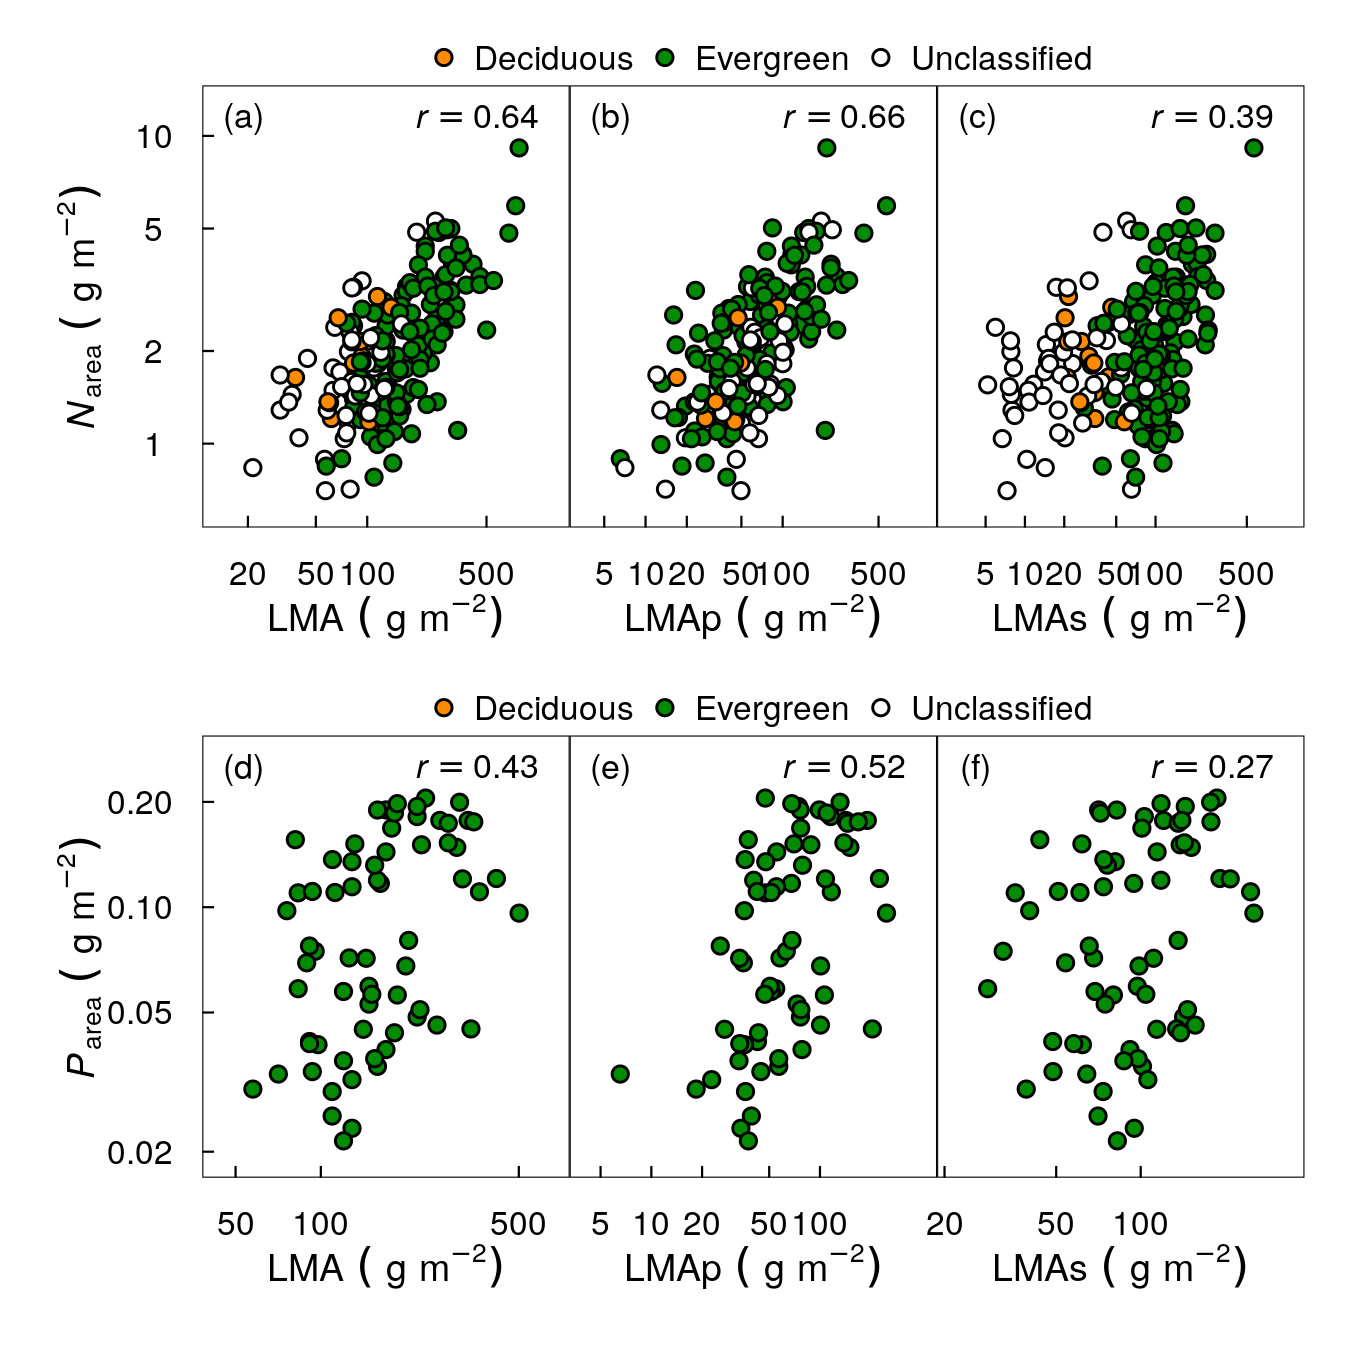
\includegraphics{../figs/gl_point_np2.pdf}

}

\caption{\label{suppfig-gl_point_np2}Measured traits related to
photosynthesis and metabolism (nitrogen and phosphorus per-unit leaf
area; \emph{N}\textsubscript{area} and \emph{P}\textsubscript{area}) are
positively correlated with LMA and with estimates (posterior medians) of
the metabolic and structural LMA components (LMAm and LMAs,
respectively) in the GLOPNET dataset. LMAm yields more consistent
relationships compared to LMA and LMAs; e.g., evergreen and deciduous
leaves align along a single relationship in panel b, but not in panels a
or c. Pearson correlation coefficients (\emph{r}) for LMA (left column)
and posterior medians of Pearson correlation coefficients (\(\bar{r}\))
for LMAm (middle column) and LMAs (right column) are shown.}

\end{suppfig}%

\newpage

\begin{suppfig}

\centering{

\includegraphics{../figs/pa_point_npc_par.pdf}

}

\caption{\label{suppfig-pa_point_npc_par}Partial regression plots for
nitrogen, phosphorus and cellulose per-unit leaf area
(\emph{N}\textsubscript{area}, \emph{P}\textsubscript{area} and
CL\textsubscript{area}). (a) LMAs variation is controlled. (b) LMAm
variation is controlled. The partial regression plots show separation
between sun and shade when controlling for LMAs variation (i.e., LMAs
does not explain the sun/shade difference), but overlapping
distributions of sun and shade when controlling for LMAm variation
(i.e., LMAm does explain the sun/shade difference). Posterior medians of
partial correlation coefficients (\(\bar{\rho}\)) are shown.}

\end{suppfig}%

\newpage

\begin{suppfig}

\centering{

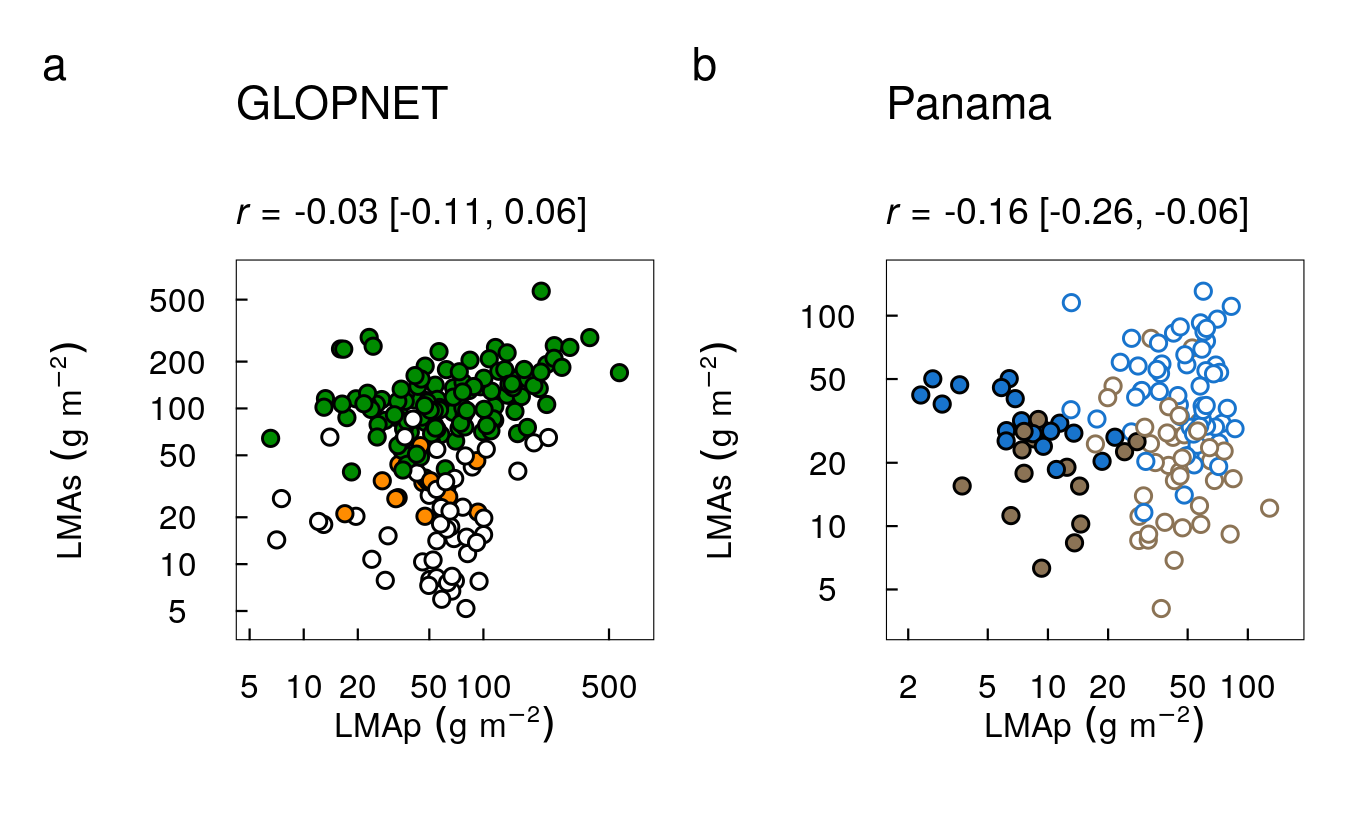
\includegraphics{../figs/ps_point.pdf}

}

\caption{\label{suppfig-LMAm_LMAs}Pearson correlation coefficients for
posterior medians of LMAm vs LMAs in the (a) GLOPNET and (b) Panama
datasets. The non-significant or weak \emph{r} values indicate that a
single axis could not accurately represent the two-dimensional space.
Symbols as in main text Figs. 2-3.}

\end{suppfig}%

\newpage

\section*{References}\label{references}
\addcontentsline{toc}{section}{References}

\phantomsection\label{refs}
\begin{CSLReferences}{1}{0}
\bibitem[\citeproctext]{ref-Alvarez2014}
Alvarez, I., Niemi, J., Simpson, M., 2014. Bayesian inference for a
covariance matrix. arXiv preprint arXiv:1408.4050v2 1--12.
\url{https://doi.org/10.1214/aos/1176348885}

\bibitem[\citeproctext]{ref-Betancourt2016}
Betancourt, M., 2016. Diagnosing {Suboptimal Cotangent Disintegrations}
in {Hamiltonian Monte Carlo}. arXiv.
\url{https://doi.org/10.48550/arXiv.1604.00695}

\bibitem[\citeproctext]{ref-Blonder2011}
Blonder, B., Violle, C., Bentley, L.P., Enquist, B.J., 2011. Venation
networks and the origin of the leaf economics spectrum. Ecology Letters
14, 91--100. \url{https://doi.org/10.1111/j.1461-0248.2010.01554.x}

\bibitem[\citeproctext]{ref-Gelman2008}
Gelman, A., Jakulin, A., Pittau, M.G., Su, Y.S., 2008. A weakly
informative default prior distribution for logistic and other regression
models. Annals of Applied Statistics 2, 1360--1383.
\url{https://doi.org/10.1214/08-AOAS191}

\bibitem[\citeproctext]{ref-Lemoine2019}
Lemoine, N.P., 2019. Moving beyond noninformative priors: Why and how to
choose weakly informative priors in {Bayesian} analyses. Oikos 128,
912--928. \url{https://doi.org/10.1111/oik.05985}

\bibitem[\citeproctext]{ref-Lewandowski2009}
Lewandowski, D., Kurowicka, D., Joe, H., 2009. Generating random
correlation matrices based on vines and extended onion method. Journal
of Multivariate Analysis 100, 1989--2001.
\url{https://doi.org/10.1016/j.jmva.2009.04.008}

\bibitem[\citeproctext]{ref-Lloyd2013}
Lloyd, J., Bloomfield, K., Domingues, T.F., Farquhar, G.D., 2013.
Photosynthetically relevant foliar traits correlating better on a mass
vs an area basis: {Of} ecophysiological relevance or just a case of
mathematical imperatives and statistical quicksand? New Phytologist 199,
311--321. \url{https://doi.org/10.1111/nph.12281}

\bibitem[\citeproctext]{ref-Osnas2018}
Osnas, J.L.D., Katabuchi, M., Kitajima, K., Wright, S.J., Reich, P.B.,
Van Bael, S.A., Kraft, N.J.B., Samaniego, M.J., Pacala, S.W., Lichstein,
J.W., 2018. Divergent drivers of leaf trait variation within species,
among species, and among functional groups. Proceedings of the National
Academy of Sciences of the United States of America 115, 5480--5485.
\url{https://doi.org/10.1073/pnas.1803989115}

\bibitem[\citeproctext]{ref-Osnas2013}
Osnas, J.L.D., Lichstein, J.W., Reich, P.B., Pacala, S.W., 2013. Global
leaf trait relationships: {Mass}, area, and the leaf economics spectrum.
Science 340, 741--744. \url{https://doi.org/10.1126/science.1231574}

\bibitem[\citeproctext]{ref-Shipley2006}
Shipley, B., Lechowicz, M.J., Wright, I., Reich, P.B., 2006. Fundamental
trade-offs generating the worldwide leaf economics spectrum. Ecology 87,
535--541. \url{https://doi.org/10.1890/05-1051}

\bibitem[\citeproctext]{ref-Westoby2013}
Westoby, M., Reich, P.B., Wright, I.J., 2013. Understanding ecological
variation across species: {Area-based} vs mass-based expression of leaf
traits. New Phytologist 199, 322--323.
\url{https://doi.org/10.1111/nph.12345}

\bibitem[\citeproctext]{ref-Wright2004a}
Wright, I.J., Reich, P.B., Westoby, M., Ackerly, D.D., Baruch, Z.,
Bongers, F., Cavender-Bares, J., Chapin, T., Cornellssen, J.H.C.,
Diemer, M., Flexas, J., Garnier, E., Groom, P.K., Gulias, J., Hikosaka,
K., Lamont, B.B., Lee, T., Lee, W., Lusk, C., Midgley, J.J., Navas,
M.L., Niinemets, Ü., Oleksyn, J., Osada, H., Poorter, H., Pool, P.,
Prior, L., Pyankov, V.I., Roumet, C., Thomas, S.C., Tjoelker, M.G.,
Veneklaas, E.J., Villar, R., 2004. The worldwide leaf economics
spectrum. Nature 428, 821--827.
\url{https://doi.org/10.1038/nature02403}

\end{CSLReferences}




\end{document}
